\chapter{Introduction: Crowdsourcing and Information Portals}
\label{cha:introduction}
\section{Motivation}

.....

\begin{figure}[!ht]
	\centering
	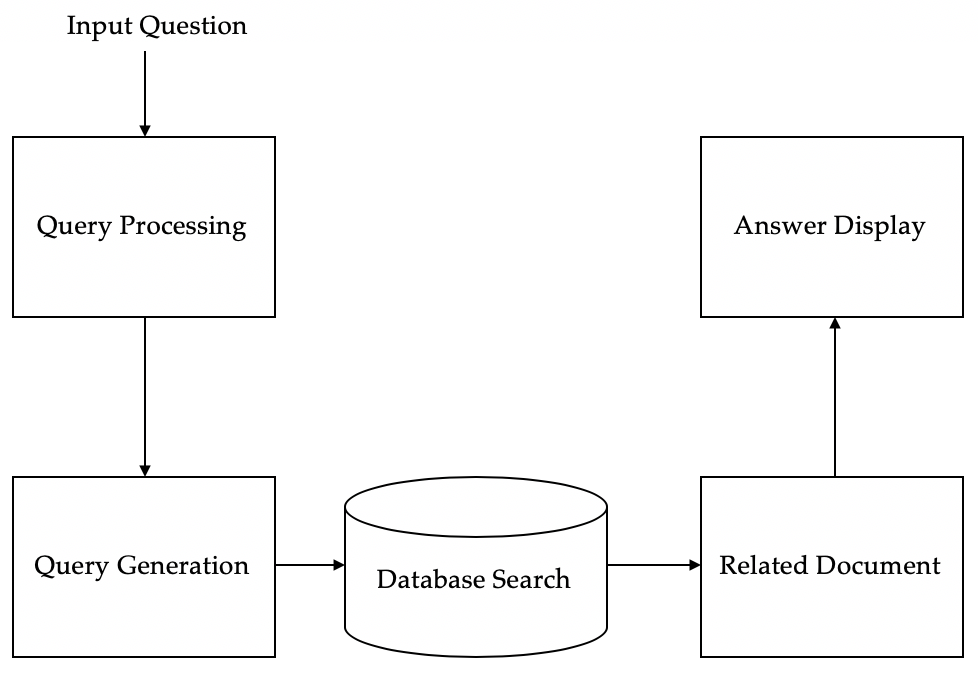
\includegraphics[width=0.5 \textwidth]{images/qa.png}\\
	\caption{A Chatbot Landscape in 2017}
    \caption*{SOURCE: KeyReply, 2017}
	\label{fig:ch1_chatbotlandscape}
\end{figure}

\section{MySections .... }
text .... Wikipedia \footnote{https://www.wikipedia.org/}

\subsection{My Subsection}
\subsubsection{My Subsubsection}
text ... 


\section{Outline}
This thesis is divided into six chapters. Chapter 1 provides an introduction to the  .... In the end, chapter 6 summarizes the results with the insights and lessons learned. 